\chapter{Results}
To ensure comparability of results obtained from each implemented method, all details related to network topologies and training process, except for those that are specific for analyzed approach, should be unified. It is especially important in case of techniques which incorporate autoencoder idea, as dimensionality of latent space, may have great impact on final results, and therefore should be kept the same for each method. Such assumptions ensure that all differences in results arise from exceptional quality of particular technique.\\

Additionally, to be able to fairly evaluate effectiveness of each implemented method, for all cases, the same set of images was used to generate final results. Images come from original dataset and were selected to cover different head positions, facial expressions and lightning conditions.

\section{Autoencoder}
The encoder and decoder XY were trained as long as there was a noticeable improvement in loss function, which in this particular case was 150 epochs, as shown in figure \ref{fig:ae_decoderXY}. If the training process would be prolonged, overfitting would occur and the encoder would lose the generalization ability.

\begin{figure}[H]
\centering
\begin{subfigure}{.5\textwidth}
  \centering
  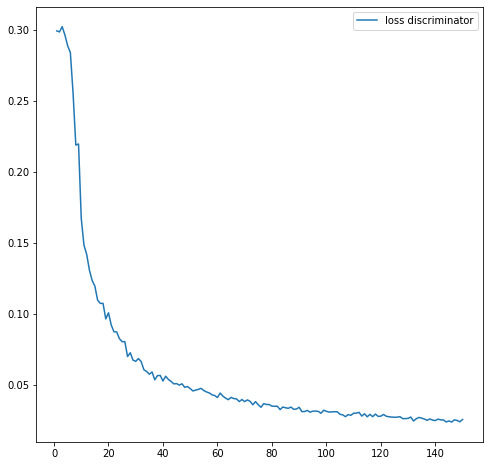
\includegraphics[width=1\linewidth]{ae_decoderXY_loss.png}
  \caption{Loss function}
  \label{subfig:ae_decoderXY_loss}
\end{subfigure}%
\begin{subfigure}{.5\textwidth}
  \centering
  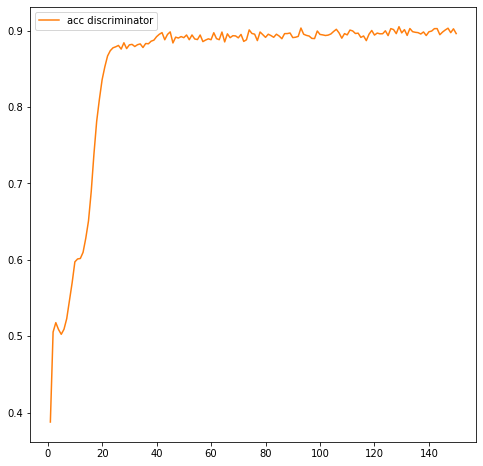
\includegraphics[width=1\linewidth]{ae_decoderXY_acc.png}
  \caption{Accuracy}
  \label{subfig:ae_decoderXY_acc}
\end{subfigure}
\caption{Training process of encoder and decoder XY}
\label{fig:ae_decoderXY}
\end{figure}

\section{Variational autoencoder}
\section{VAE-GAN}
\section{CycleGAN}